\subsection{Trackpy}
\label{sec:locate:trackpy}

Trackpy~\cite{trackpy} is a particle tracking library developed by Soft Matter.
Its \texttt{Locate} function performs the task required, if an extra output format transformation step is applied.

\subsubsection{Algorithm}

As described in the documentation, the \texttt{Locate} function implements the following algorithm:
\begin{enumerate}
	\itemsep 0em
	\item Pre-process the image by performing a band pass and a threshold.
	\item Locate all peaks of brightness, characterize the neighborhoods of the peaks and take only those with given total brightness (``mass'').
	\item Refine the positions of each peak.
\end{enumerate}

\subsubsection{Evaluation}

As displayed in figure~\ref{fig:locate:trackpy}, the algorithm performed well on quality, finding about 85\% of the tracers, but with some strange offset in the positions.
The speed was however extremely low, at just 3 FPS.

\begin{figure}
	\centerline{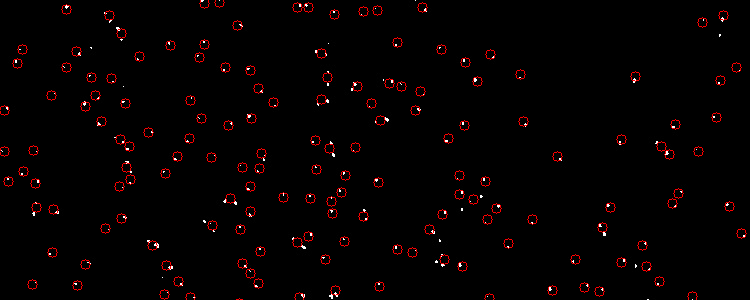
\includegraphics[width=\locateimgsize]{images/locate/trackpy.png}}
	\caption{\centering Trackpy's result}
	\label{fig:locate:trackpy}
\end{figure}
